%
% $File: report.tex
% $Date: Fri Jan 03 17:05:17 2014 +0800
%

\documentclass{article}
\usepackage{fontspec}
\usepackage{zhspacing,url,amsmath,amssymb,verbatim}
\usepackage{pdfpages}
\zhspacing
\usepackage{listings}
\usepackage[hyperfootnotes=false,colorlinks,linkcolor=blue,anchorcolor=blue,citecolor=blue]{hyperref}
\usepackage[backend=biber]{biblatex}
\usepackage{graphicx}
\usepackage{minted}
\usepackage{subfigure}
\usepackage{indentfirst}
\usepackage{cases}
\usepackage{float}			% don't automatically change location of figure [H]
\usepackage{chngpage}		% use \changetext to change page size
\usepackage{environ}
\usepackage{array}
\usepackage[top=1in, bottom=1in, left=1.25in, right=1.25in]{geometry}
\usepackage{caption}\captionsetup{hypcap=true}  % ref to jump to object instead of caption
\newfontfamily\zhfont[BoldFont=SimHei,ItalicFont=KaiTi_GB2312]{SimSun}
\lstset{keywordstyle=\color{blue!70}, commentstyle=\color{red!50!green!50!blue!50},frame=shadowbox,rulesepcolor=\color{red!20!green!20!blue!20},
basicstyle=\footnotesize\ttfamily}

\setlength{\parindent}{2em}

% $File: mint-defs.tex
% $Date: Thu Sep 26 22:11:33 2013 +0800
% $Author: Xinyu Zhou <zxytim@gmail.com>

\newcommand{\inputmintedConfigured}[3][]{\inputminted[fontsize=\footnotesize,
	label=#3,linenos,frame=lines,framesep=0.8em,tabsize=4,#1]{#2}{#3}}

\newcommand{\txtsrc}[2][]{\inputmintedConfigured[#1]{text}{#2}}
\newcommand{\txtsrcpart}[4][]{\txtsrc[firstline=#3,firstnumber=#3,lastline=#4,#1]{#2}}

\newcommand{\cppsrc}[2][]{\inputmintedConfigured[#1]{cpp}{#2}}
\newcommand{\cppsrcpart}[4][]{\cppsrc[firstline=#3,firstnumber=#3,lastline=#4,#1]{#2}}

\newcommand{\javasrc}[2][]{\inputmintedConfigured[#1]{java}{#2}}
\newcommand{\javasrcpart}[4][]{\javasrc[firstline=#3,firstnumber=#3,lastline=#4,#1]{#2}}

\newcommand{\matlabsrc}[2][]{\inputmintedConfigured[#1]{matlab}{#2}}
\newcommand{\matlabsrcpart}[4][]{\matlabsrc[firstline=#3,firstnumber=#3,lastline=#4,#1]{#2}}

%\usepackage[T1]{fontenc}
\usepackage{lmodern}
\usepackage{amssymb,amsmath}
\usepackage{ifxetex,ifluatex}
\usepackage{fixltx2e} % provides \textsubscript
% use upquote if available, for straight quotes in verbatim environments
\IfFileExists{upquote.sty}{\usepackage{upquote}}{}
\ifnum 0\ifxetex 1\fi\ifluatex 1\fi=0 % if pdftex
  \usepackage[utf8]{inputenc}
\else % if luatex or xelatex
  \usepackage{fontspec}
  % commented by Xinyu Zhou
  \ifxetex
    \usepackage{xltxtra,xunicode}
  \fi
  \defaultfontfeatures{Mapping=tex-text,Scale=MatchLowercase}
  \newcommand{\euro}{€}
\fi
% use microtype if available
\IfFileExists{microtype.sty}{\usepackage{microtype}}{}
\usepackage{color}
\usepackage{fancyvrb}
\newcommand{\VerbBar}{|}
\DefineShortVerb[commandchars=\\\{\}]{\|}
\DefineVerbatimEnvironment{Highlighting}{Verbatim}{commandchars=\\\{\}}
% Add ',fontsize=\small' for more characters per line
\newenvironment{Shaded}{}{}
\newcommand{\KeywordTok}[1]{\textcolor[rgb]{0.00,0.44,0.13}{\textbf{{#1}}}}
\newcommand{\DataTypeTok}[1]{\textcolor[rgb]{0.56,0.13,0.00}{{#1}}}
\newcommand{\DecValTok}[1]{\textcolor[rgb]{0.25,0.63,0.44}{{#1}}}
\newcommand{\BaseNTok}[1]{\textcolor[rgb]{0.25,0.63,0.44}{{#1}}}
\newcommand{\FloatTok}[1]{\textcolor[rgb]{0.25,0.63,0.44}{{#1}}}
\newcommand{\CharTok}[1]{\textcolor[rgb]{0.25,0.44,0.63}{{#1}}}
\newcommand{\StringTok}[1]{\textcolor[rgb]{0.25,0.44,0.63}{{#1}}}
\newcommand{\CommentTok}[1]{\textcolor[rgb]{0.38,0.63,0.69}{\textit{{#1}}}}
\newcommand{\OtherTok}[1]{\textcolor[rgb]{0.00,0.44,0.13}{{#1}}}
\newcommand{\AlertTok}[1]{\textcolor[rgb]{1.00,0.00,0.00}{\textbf{{#1}}}}
\newcommand{\FunctionTok}[1]{\textcolor[rgb]{0.02,0.16,0.49}{{#1}}}
\newcommand{\RegionMarkerTok}[1]{{#1}}
\newcommand{\ErrorTok}[1]{\textcolor[rgb]{1.00,0.00,0.00}{\textbf{{#1}}}}
\newcommand{\NormalTok}[1]{{#1}}
% \ifxetex
%   \usepackage[setpagesize=false, % page size defined by xetex
%               unicode=false, % unicode breaks when used with xetex
%               xetex]{hyperref}
% \else
%   \usepackage[unicode=true]{hyperref}
% \fi
\hypersetup{breaklinks=true,
            bookmarks=true,
            pdfauthor={},
            pdftitle={},
            colorlinks=true,
            urlcolor=blue,
            %linkcolor=magenta,
            pdfborder={0 0 0}}
%\urlstyle{same}  % don't use monospace font for urls
\setlength{\parindent}{0pt}
\setlength{\parskip}{6pt plus 2pt minus 1pt}
\setlength{\emergencystretch}{3em}  % prevent overfull lines
%\setcounter{secnumdepth}{0}



\newcommand{\figref}[1]{\hyperref[fig:#1]{Figure.\ref*{fig:#1}}}
\newcommand{\tableref}[1]{\hyperref[table:#1]{Table.\ref*{table:#1}}}
\newcommand{\centerize}[1]{\begin{center} #1 \end{center}}
\newcommand{\secref}[1]{\hyperref[sec:#1]{Section.\ref*{sec:#1}}}
\newcommand{\appref}[1]{\hyperref[app:#1]{App.\ref*{app:#1}}}


\usepackage{fancyhdr}
\changetext{}{2.2cm}{-1.1cm}{-1.1cm}{}
\pagestyle{fancy}
\setlength{\headheight}{15.2pt}
\lhead[]{}\rhead[]{}
\fancyhead[C]{\emph{Speaker Recognition}}

% math function
\let\Oldsum\sum
\renewcommand{\sum}{\displaystyle\Oldsum}
\let\Oldprod\prod
\renewcommand{\prod}{\displaystyle\Oldprod}


\newcommand{\cmd}[1]{{\it #1}}
\newcommand{\ccmd}[1]{\centerize{\cmd{#1}}}

\title{Digital Signal Processing: Speaker Recognition \\ Final Report \\ Complete Version}
\author{Xinyu Zhou, Yuxin Wu, and Tiezheng Li\\ Tsinghua University}
\date{}

\bibliography{refs.bib}
\begin{document}

\fontsize{11pt}{1.4em}
\setlength{\baselineskip}{1.6em}
\maketitle


\section{Introduction}
A \textbf{Speaker Recognition} tasks can be classified with respect to different criterion:
Text-dependent or Text-independent, Verification (decide whether the person is he claimed to be) or Identification (decide who the person is by its voice).\cite{SRwiki}

Speech is a kind of complicated signal produced as a result of several transformations occurring at different levels: semantic, linguistic and acoustic.
Differences in these transformations may lead to differences in the acoustic properties of the signals.
The recognizability of speaker can be affected not only by the linguistic message
but also the age, health, emotional state and effort level of the speaker.
Background noise and performance of recording device also interfere
the classification process.

Speaker recognition is an important part of Human-Computer Interaction (HCI).
As the trend of employing wearable computer reveals,
Voice User Interface (VUI) has been a vital part of such computer.
As these devices are particularly small, they are more likely to lose and be stolen.
In these scenarios, speaker recognition is not only a good HCI,
but also a combination of seamless interaction with computer and security guard
when the device is lost.
The need of personal identity validation will become more acute in the future.
Speaker verification may be essential in business telecommunications.
Telephone banking and telephone reservation services will develop rapidly
when secure means of authentication were available.

Also,the identity of a speaker is quite often at issue in court cases.
A crime victim may have heard but not seen the perpetrator,
but claim to recognize the perpetrator as someone whose voice was previously familiar;
or there may be recordings of a criminal whose identity is unknown.
Speaker recognition technique may bring a reliable scientific determination.

Furthermore, these techniques can be used in environment which demands high security.
It can be combined with other biological metrics to form a multi-modal authentication system.

In this task, our goal is to build a proof-of-concept text-dependent speaker recognition system with GUI support.
Hopefully, we would like to extend its ability to a text-independent speaker recognition system.

%File: algorithm.tex
%Date: Sun Nov 17 23:43:49 2013 +0800
%Author: Yuxin Wu <ppwwyyxxc@gmail.com>

\section{Algorithm and Implementation}

We presented a prototype system based on MFCC as acoustic features, and
GMM as our recognition model.

\subsection{MFCC}
MFCC (Mel-frequency Cepstral Coefficient) is a representation of the short-term power spectrum of a sound,
based on a linear cosine transform of a log
power spectrum on a nonlinear mel-scale of frequency \cite{mfcc} .
MFCC is the mostly widely used features in Automatic Speech Recognition(ASR), and it can also be
applied to Speaker Recognition task.

The process to extract MFCC feature is as followed:
\begin{figure}[H]
  \centering
  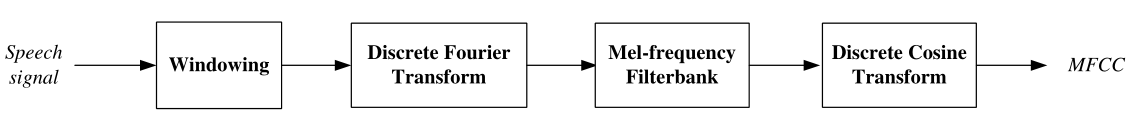
\includegraphics[width=\textwidth]{res/MFCC.png}
\end{figure}

First, the input speech should be divided into successive short-time frames of length $L$,
neighboring frames shall have overlap $R$. In our implementation, We choose $L = 20ms  $ ans $ R = 10 ms$.
Those frames are then windowed by Hamming Window, as shown in \figref{frames}
\begin{figure}[H]
  \centering
  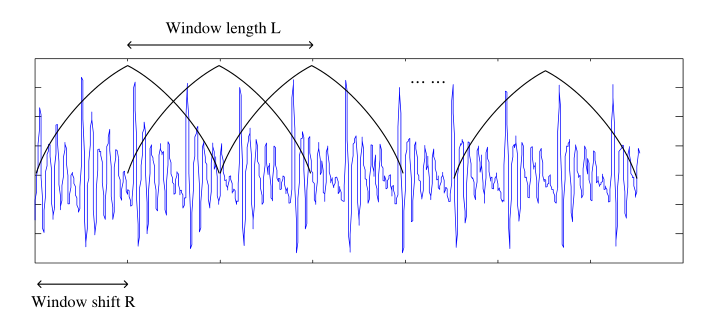
\includegraphics[width=0.7\textwidth]{res/frames.png}
  \caption{Framing and Windowing \label{fig:framming}}
\end{figure}

Then, We perform Discrete Fourier Transform (DFT) on windowed signals to compute their spectrums.
For each of $N$ discrete frequency bands we get a complex number $X[k]$ representing
magnitude and phase of that frequency component in the original signal.

Considering the fact that human hearing is not equally sensitive to all frequency bands, and especially, it has lower resolution at higher frequencies.
Scaling methods like Mel-scale and Bark-scale are aimed at scaling the frequency domain to fit human auditory perception better.
They are approximately linear below 1 kHz and logarithmic above 1 kHz.
\begin{figure}[H]
  \centering
  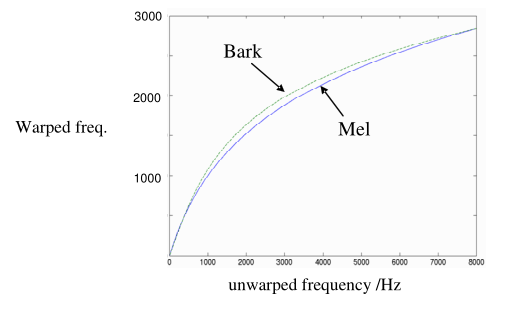
\includegraphics[width=0.6\textwidth]{res/mel-scale.png}
\end{figure}

In MFCC, Mel-scale is applied on the spectrums of the signals. The expression of Mel-scale warpping is as followed:
\[ M(f) = 2595 \log_{10}(1 + \dfrac{f}{700}) \]

\begin{figure}[H]
  \centering
  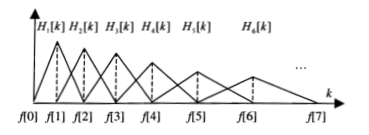
\includegraphics[width=0.5\textwidth]{res/bank.png}
  \caption{Filter Banks (6 filters) \label{fig:bank}}
\end{figure}
Then,  we appply the bank of filters according to Mel-scale on the spectrum,
calculate the logarithm of energy under each bank by $E_i[m] = \log (\sum_{k=0}^{N-1}{X_i[k]^2 H_m[k]}) $ and apply Discrete
Cosine Transform (DCT) on $E_i[m](m = 1, 2, \cdots M) $ to get an array $c_i $:
\[ c_i[n] = \sum_{m=0}^{M-1}{E_i[m]\cos(\dfrac{\pi n}{M}(m - \dfrac{1}{2}))} \]

Usually, the first 13 terms in $c_i $ is used as features for future training.

\subsection{GMM}

We use Gaussian Mixture Model (GMM) to model all features from one person.
For implementation, we use the GMM model training and predicting routine from the famous python
machine learning package scikit-learn \cite{sklearn}.
Since the last step of MFCC is DCT, different dimensions of the features are strongly independent, so we
use GMM with diagonal covariance matrix. The number of components in GMM is chosen as 32 in our implementation.

After building models for each person, it can be used to calculate the probability that the input signal is generated by this model.
The model with maximum probability is picked out as the result, and the corresponding person is recognized.

\pysrcpart{res/test.py}{45}{50}

%File: implementation.tex
%Date: Fri Jan 03 21:51:56 2014 +0800


\section{Implementation}
The whole system is written mainly in python, together with some code in C++ and matlab.
The system strongly relies on the support of the numpy\cite{numpy} and scipy\cite{scipy} library.

\begin{enumerate}
    \item VAD

      Three types of  VAD filters are located in \verb|src/filters/|.

      \verb|silence.py| implements an energy-based VAD algorithm.
      \verb|ltsd.py| is a wrapper for LTSD algorithm, relying on pyssp\cite{pyssp}.
      \verb|noisered.py| is a wrapper for SOX noise reduction tools, relying on SOX \cite{sox} being
      installed in the system.

    \item Feature

      Implementations for feature extraction are locaed in \verb|src/feature/|.

      \verb|MFCC.py| is a self-implemented MFCC feature extractor.
      \verb|BOB.py| is a wrapper for the MFCC feature extraction in the bob \cite{bob2012} library.
      \verb|LPC.py| is a LPC feature extractor, relying on \verb|scikits.talkbox| \cite{talkbox}.
      All the three extractor have the same interface, with configurable parameters.

      In the implemention, we have  tried different parameters of these features.
      The test script can be found as \verb|src/test/test-feature.py|
      According to our experiments, we have found that the following parameters are optimal:
      \begin{itemize}
        \item Common parameters:
          \begin{itemize}
            \item Frame size: 32ms
            \item Frame shift: 16ms
            \item Preemphasis coefficient: 0.95
          \end{itemize}
        \item MFCC parameters:
          \begin{itemize}
            \item number of cepstral coefficient: 15
            \item number of filter banks: 55
            \item maximal frequency of the filter bank: 6000
          \end{itemize}
        \item LPC Parameters:
          \begin{itemize}
            \item number of coefficient: 23
          \end{itemize}
      \end{itemize}

    \item GMM

      We have tried GMM from scikit-learn \cite{scikit-learn} as well as pypr \cite{pypr}, but
      they suffer a common problem of inefficency.
      For the consideration of speed, a C++ version of GMM with K-MeansII initialization and
      concurrency support
      was implemented and located in \verb|src/gmm/|. It requires \verb|g++>=4.7| to compile.
      This implementation of GMM also provides a python binding which have similar interface to the GMM in
      scikit-learn.

      The new version of GMM, has enhancement in both speed and accuracy. A more detailed discussion
      will be in \secref{result}.

      At last, we used GMM with 32 components, which is found to be optimal according to our experiment.
      The covariance matrix of every Gaussian component is assumed to be diagonal,
      since each dimension of the feature vector are independent.

    \item CRBM

      CRBM is implemented in C++, located in \verb|src/nn|. It also has concurrency support.

    \item JFA

      From our investigation, we found that the original algorithm \cite{jfa-se} for training JFA model is of
      too much complication and hard to implement.
      Therefore, we use the simpler algorithm presented in \cite{jfa-study}
      to train the JFA model.
      This JFA implementation is based on JFA cookbook\cite{cookbook}.
      To generate feature files for JFA, \verb|test/gen-features-file.py| shall be used.
      After \verb|train.lst, test.lst, enroll.lst| are properly located in \verb|jfa/feature-data|,
      the script \verb|run_all.m| will do the training and testing, and \verb|exp/gen_result.py|
      will calculate the accuracy.

      However, from the result, JFA does not seem to outperform our enhanced MFCC and GMM algorithms
      (but do outperform our old algorithms). It is suspected that the training of a JFA model needs more data than
      we have provided, since JFA needs data from various source to account for different types of variabilities.
      Therefore, we might need to add extra data on the training of JFA, but keep the same data scale in the stage of enrollment,
      to get a better result.

      It is also worth mentioning that the training of JFA will take much longer time than our old method,
      since the estimation process of $ u, v, d$ does not converge quickly. As a result, it might not be practical to add
      JFA approach to our GUI system. But we will still test further on the performance of it, compared to other methods.

    \item GUI

      GUI is implemented based on PyQt\cite{pyqt} and PyAudio\cite{pyaudio}.
      \verb|gui.py| is the entrance point. The usage of GUI will be introduced in \secref{gui}.
  \end{enumerate}


\section{Dataset}
	The dataset provided by teacher comprised of 102 speaker, in which 60 are
	females and the rest are males, with three different speaking style: Spontaneous,
	Reading and Whisper. A statistic is as follows:
	\begin{table}[!ht]
		\centering
		\begin{tabular}{|c|c|c|c|}
			\hline
			& Spontaneous & Reading & Whisper \\\hline
			Average Duration & 202s & 205s & 221s \\\hline
			Female Average Duration & 205s & 202s & 217s \\\hline
			Male Average Duration & 200s & 203s & 223s \\\hline
		\end{tabular}
	\end{table}

\section{Performance}
\label{sec:result}
We have tested our approaches under various parameters, based on a corpus provided by teacher Xu.
For detailed description of the corpus, please see former report.

All the tests in this section have been conducted serval times
(depending on computation cost, vary from 10 to 30)
with random selected training and testing speakers.
The average over these tests are considered as confidential result.

%\subsection{Efficiency Test of our GMM}
%We have extensively examined the efficiency of our implementation of GMM
%compared to scikit-learn version. Test is conducted using real MFCC data with
%13 dimensions. We consider the scenario when training a UBM with 256 mixtures.
%We examine the time used for ten iteration.  For comparable results, we diabled
%the K-means initialization process of both scikit-learn GMM implementation and
%ours.  Time used for ten iterations under different data size and concurrency
%is recorded.

%From \figref{gmm_efficiency}, we can immediately infer that our method
%is much-much more efficient than the widely used version of GMM provided
%by scikit-learn when the data size grows sufficiently large.

%We shall analyze in two aspect:
%\begin{itemize}
	%\item No concurrency
		%\begin{itemize}
			%\item When the number of MFCC features is below 6000, which is a typical
				%number of features generated by 60 seconds utterances (1ms frame shift),
				%our method is slightly slower; but this is trivial since
				%1 minute utterance is too small.
			%\item When the number of MFCC features grows sufficiently large, our method
				%shows great improvement. When training 512,000 features, our method
				%is 5 times faster than comparing method.
		%\end{itemize}
	%\item With concurrency \\
		%Our method shows considerable concurrency scalability that the running time
		%is approximately lineary to the number of cores using.

		%When using 8-cores, our method is \textbf{$19$ times} faster than comparing
		%method.
%\end{itemize}


\subsection{Change in MFCC Parameters}
\begin{enumerate}
    \item Different Number of Cepstrums

      \item Different Number of Filterbanks

        \item Different Size of Frame
\end{enumerate}

\subsection{Change in LPC Parameters}
\begin{enumerate}
    \item Different Number of Coefficient

        \item Different Size of Frame
\end{enumerate}

\subsection{Change in GMM Components}

We examined our GMM compared to GMM from scikit-learn.
Test is conducted on 30-speaker corpus, 30 seconds training utterance
and 100 random sampled 5 seconds test utterance for each speaker.

As \figref{mixture} illustrates, when number of mixtures is small,
our GMM outperforms scikit-learn version by $10\%$, which indicates our
GMM models the distribution more accurately. The maximum accuracy
happens when the number of mixtures is around 32, reaching $0.965$. As
the number of mixtures increases, the decrease in accuracy

\subsection{Performance with Well-Tuned Parameters}

An apparent trade-off in speaker recognition task is the number of speakers
enrolled and the accuracy on recognization.
Also, the duration of signal for enrollment and test can have significant effect on the accuracy.
We've conducted test using well-tuned parameters for feature extraction and GMM, on dataset with
various number of people and with various test duration.

The configurations of this experiment is as followed:
\begin{itemize}
  \item MFCC: frame size is $32 ms $, 19 cepstrums, 55 filterbanks
  \item LPC: frame size is $32 ms $, 15 coefficients
  \item GMM from scikit-learn, number of mixtures is 32
  \item 20s utterance for enrollment
  \item 50 sampled test utterance for each user
\end{itemize}


Scrunitizing \figref{nspk_enrolled} we would see that, our GMM performs better than
scikit GMM in general. When number of speakers is small, due to the random
selection, the variance of the tests is significantly high, as we can see from the curve fluctuants.
When number of speakers increases, it is clear that the
accuracy of our GMM is above scikit version. As the more speaker, the more
difficult the recognition task will be, this result suggests that our
optimization on GMM takes effect.



\section{GUI}
\label{sec:gui}
The GUI contains following tabs:
\begin{itemize}
  \item \textbf{Enrollment} \\

    \begin{figure}[H]
      \centering
      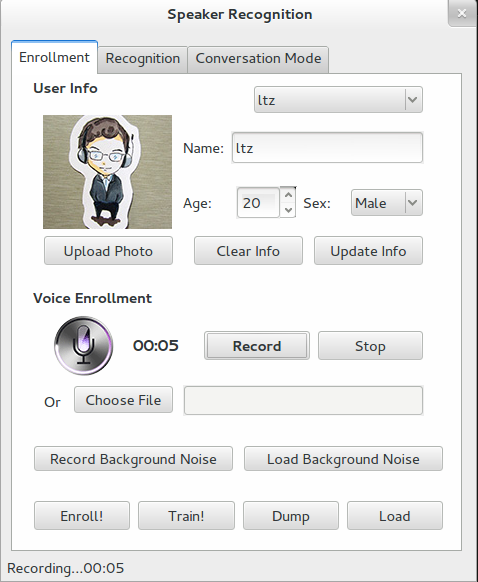
\includegraphics[width=0.8\textwidth]{img/enrollment.png}
    \end{figure}

    A new user may start his or her first step by clicking the
    tab Enrollment. New users could provide personal information
    such as name, sex, and age. then upload personal avatar to
    build up their own data. Experienced users can choose from
    the userlist and update their infomation.

    Next the user needs to provide a piece of utterance for
    the enrollment and training process.

    There are two ways to enroll a user:
    \begin{itemize}
      \item \textbf{Enroll by Recording}
        Click Record and start talking while click Stop to stop
        and save.There is no limit of the content of the utterance,
        whileit is highly recommended that the user speaks long enough
        to provide sufficient message for the enrollment.

      \item \textbf{Enroll from Wav Files}
        User can upload a pre-recorded voice of a speaker.(*.wav recommended)
        The systemaccepts the voice given and the enrollment of a speaker is done.
    \end{itemize}

    The user can train, dump or load his/her voice features after enrollment.

  \item \textbf{Recognition of a user} \\
    \begin{figure}[H]
      \centering
      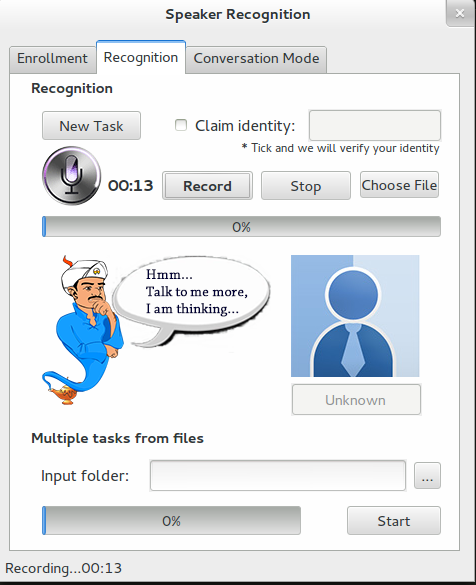
\includegraphics[width=0.8\textwidth]{img/recognition.png}
    \end{figure}

    A enrolled user present or record a piece of utterance,
    the system tells who the person is and show user's avatar.
    Recognition of multiple pre-recorded files can be done as well.

  \item \textbf{Conversation Recognition Mode} \\
    \begin{figure}[H]
      \centering
      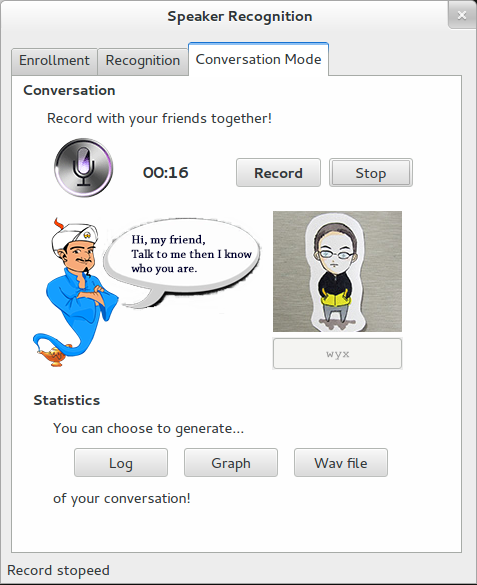
\includegraphics[width=0.8\textwidth]{img/conversation.png}
      \caption{\label{fig:}}
    \end{figure}

    In Conversation Recognition mode, multiple users can have conversations
    together near the microphone. Same recording procedure as above.
    The system will continuously collect voice data, and determine
    who is speaking right now. Current speaker's anvatar will show up
    in screen; otherwise the name will be shown. The conversation
    audio can be downloaded and saved.
    There are some ways to visualize the speaker-distribution in the
    conversation.
    \begin{itemize}
      \item \textbf{Conversation log}
        A detailed log, including start time, stop time,
        current speaker of each period is generated.
      \item \textbf{Conversation flow graph}
        \begin{figure}[H]
          \centering
          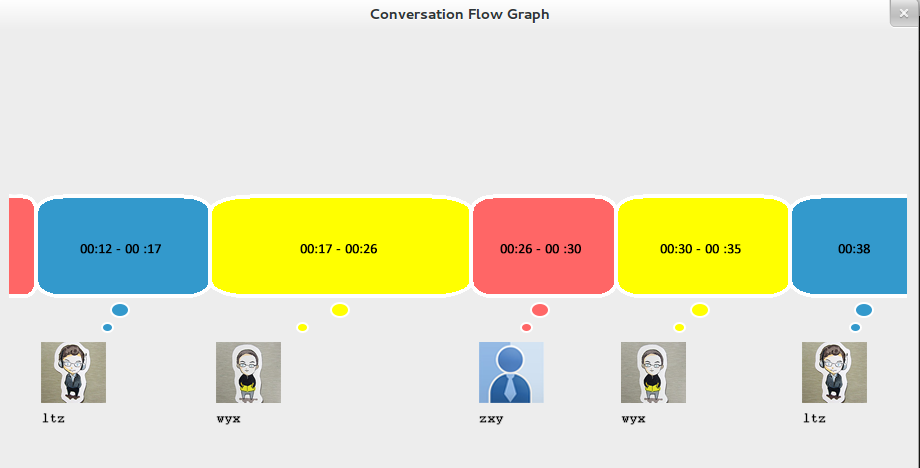
\includegraphics[width=0.8\textwidth]{img/conversationgraph.png}
        \end{figure}

        A timeline of the conversation will be shown by a number of
        talking-clouds joining together, with start time, stop time
        and users' avatars labeled. Different users are presented
        with different colors.The timeline will flow to the left dynamically
        just as time elapses. The visualization of the conversation is done
        in this way. This functionality is still under development.
    \end{itemize}

\end{itemize}


\printbibliography

\end{document}

